\section{Listener\-Object Class Reference}
\label{classListenerObject}\index{ListenerObject@{ListenerObject}}
Inheritance diagram for Listener\-Object::\begin{figure}[H]
\begin{center}
\leavevmode
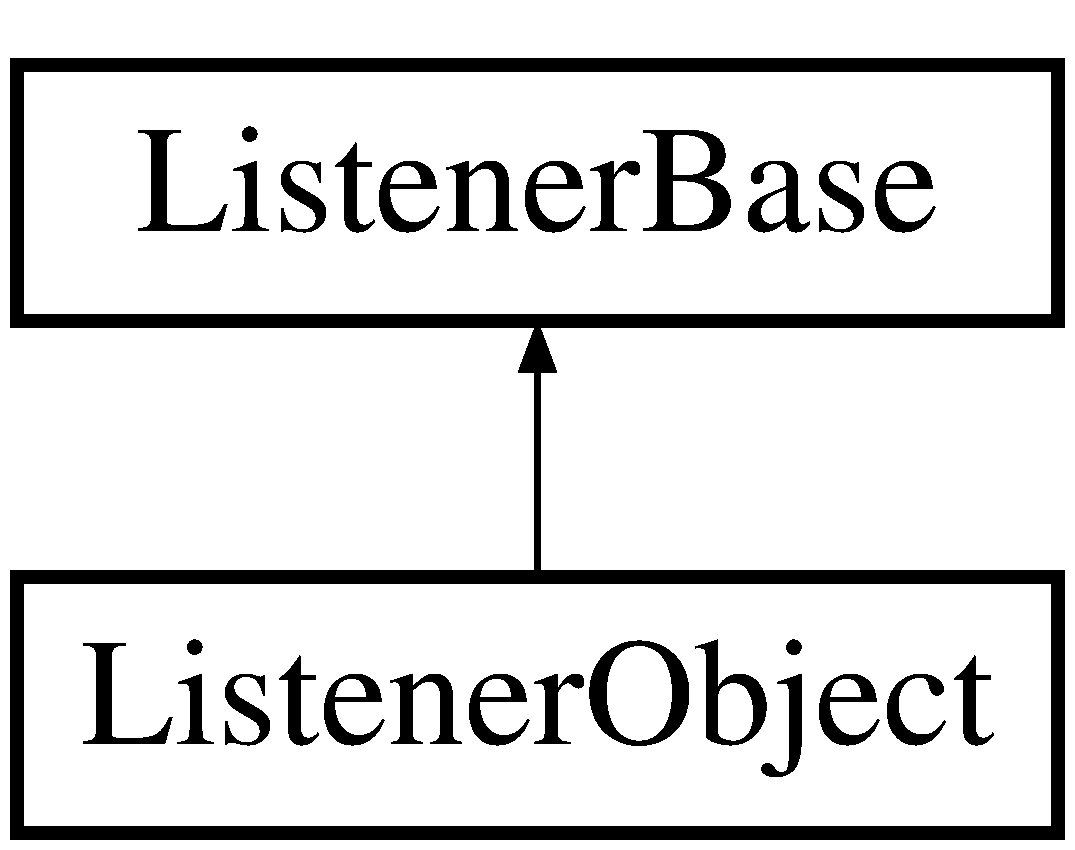
\includegraphics[height=2cm]{classListenerObject}
\end{center}
\end{figure}
\subsection*{Public Member Functions}
\begin{CompactItemize}
\item 
{\bf invoke} ()
\end{CompactItemize}


\subsection{Member Function Documentation}
\index{ListenerObject@{Listener\-Object}!invoke@{invoke}}
\index{invoke@{invoke}!ListenerObject@{Listener\-Object}}
\subsubsection{\setlength{\rightskip}{0pt plus 5cm}Listener\-Object::invoke ()}\label{classListenerObject_ListenerObjecta0}




Reimplemented from {\bf Listener\-Base} {\rm (p.\,\pageref{classListenerBase_ListenerBasea0})}.

The documentation for this class was generated from the following file:\begin{CompactItemize}
\item 
{\bf Listener.py}\end{CompactItemize}
